
\documentclass{standalone}

\usepackage{amsmath} 
\usepackage{tikz}

\begin{document}
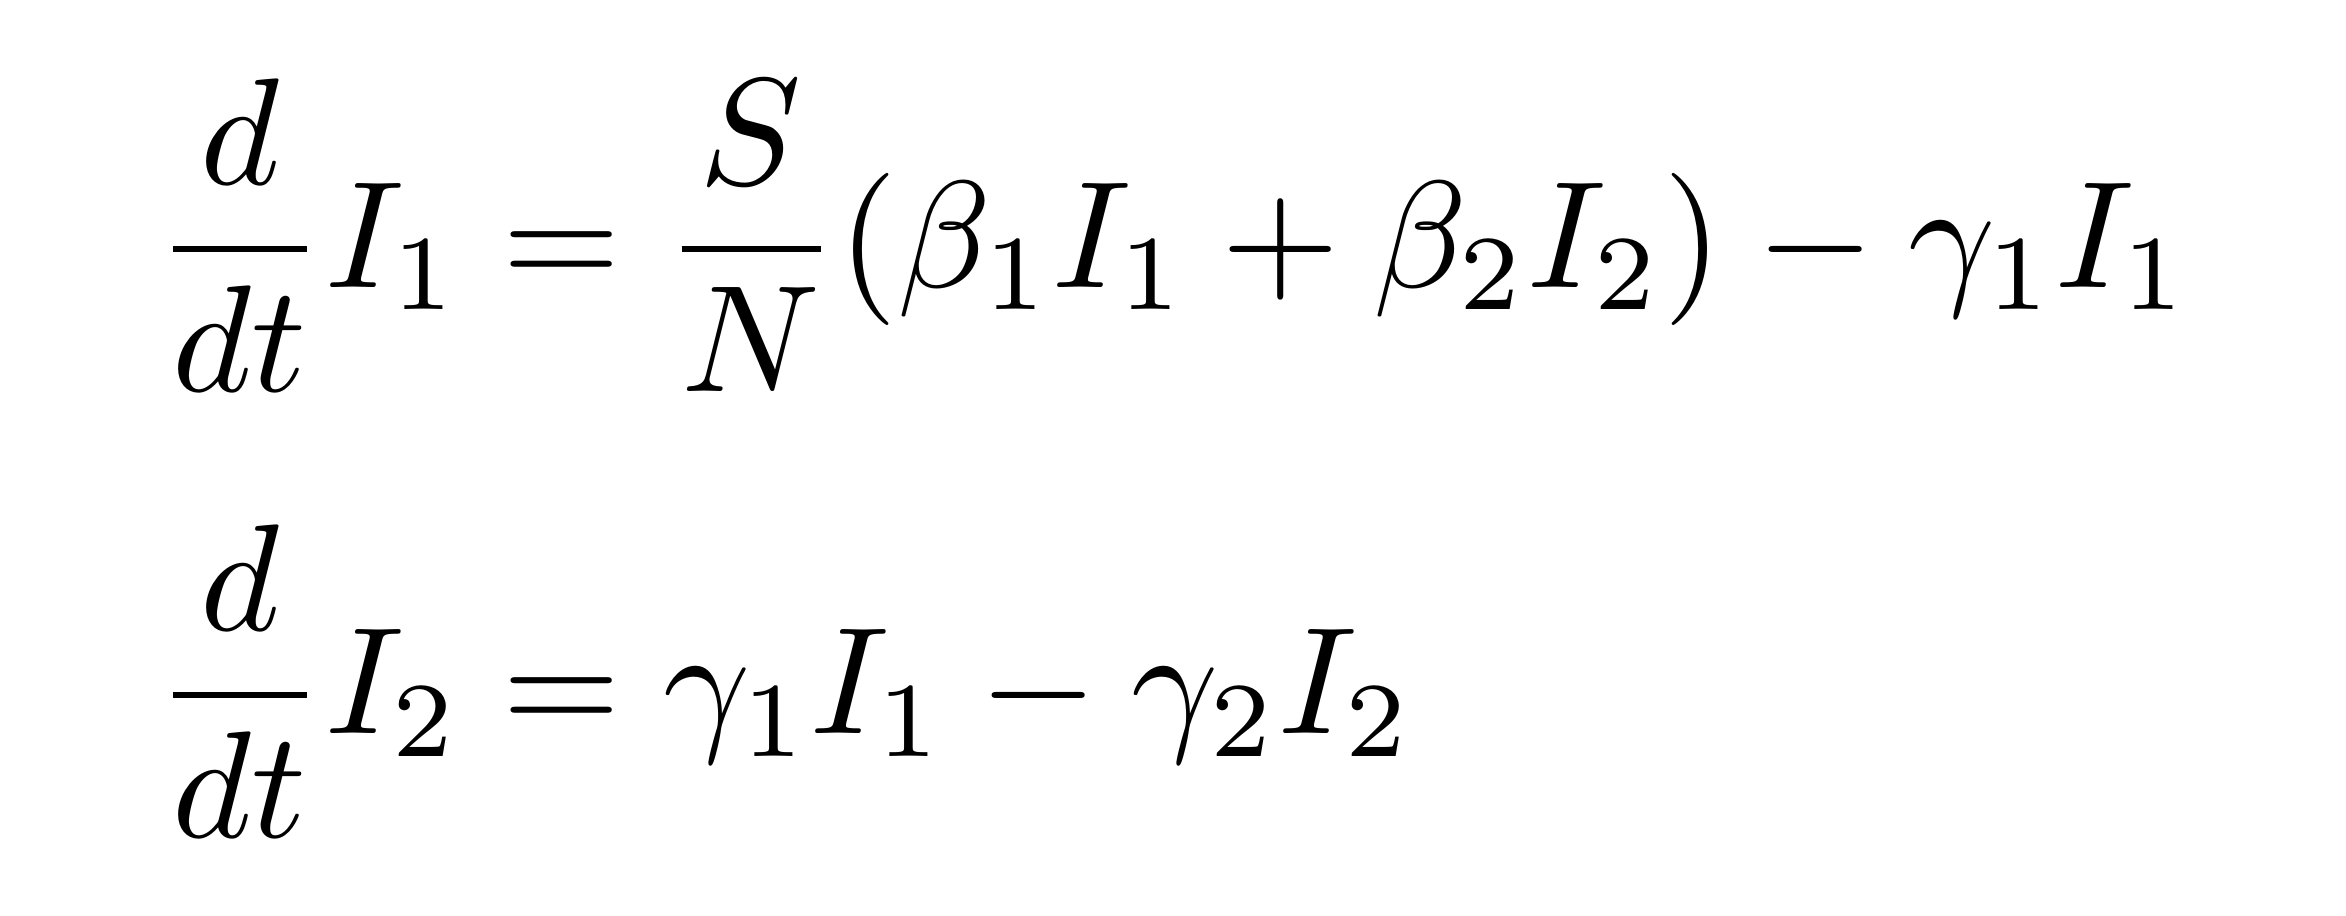
\begin{tikzpicture}
\node[scale=5.5] {
$
\begin{array}{l}
\dfrac{d}{dt}I_1 =  \dfrac{S}{N} (\beta_1  I_1 + \beta_2  I_2) - \gamma_1 I_1  \\[\bigskipamount]
\dfrac{d}{dt}I_2  =  \gamma_1 I_1- \gamma_2 I_2   
\end{array}
$
};
\end{tikzpicture}
\end{document}


%\begin{tikzpicture}
%\node[scale=8.0] {
%$\begin{aligned}
%\frac{d}{dt}I_1 &=  \frac{S}{N} (\beta_1  I_1 + \beta_2  I_2) - \gamma_1 I_1  \\
%\frac{d}{dt}I_2 &=  \gamma_1 I_1- \gamma_2 I_2   \\
%%%\frac{\partial I_1}{\partial t} &=  \frac{S}{N} (\beta_11 I_1 + \beta_21 I_2) - \gamma_1 I_1  \\
%%%\frac{\partial I_2}{\partial t} &=  \gamma_1 I_1- \gamma_2 I_2 
%\end{aligned}$
%};
%\end{tikzpicture}